%==========================================================================
\chapter{Conceptual Interfaces for Inputting Problem Data}
\label{Conceptual Interfaces}

\section{What do we mean by ``conceptual interfaces?''}

In Figure \ref{fig-conceptual-interface} we present an illustration
of the philosophy behind conceptual interfaces.

[Cut and paste from Rob's paper].

\begin{figure}
\centering
\includegraphics[width=5in]{concep_iface.eps}
\caption{%
Graphic illustrating the notion of conceptual interfaces.}
\label{fig-conceptual-interface}
\end{figure}

\section{Which conceptual interface should I use?}

